% !TeX root = ../main.tex

% Edit this title for each week's entry.
\section{Week 4 - Risk, Reward and Arbitrage}

\topic{Capital Asset Pricing Model}

\begin{definition}[Valuation]
    The analytical process of determining the current (or projected) worth
    of an asset or a company. A valuation has two components:
    \begin{itemize}
        \item \b{Projected cash-flows}
        \item \b{Interest rate}: determined by risk (uncertainty)
    \end{itemize}
\end{definition}
Engineers often need project valuations to make decisions, e.g.\ lease or
buy, replace or keep current equipment, go or no-go on a project.

\heading{Why Proper Valuations Are Important}
Auger and Guzman (2010) looked at 51 copper-mining investments (1957--1999):
\begin{itemize}
    \item Half of the projects were invested in at a sub-optimal time
    \item 36 projects should have been designed with a 40\% larger or smaller capacity
    \item Sub-optimal decisions led to a total NPV \b{49\% lower} than optimal
\end{itemize}
\db{Conclusion: use better valuation methods (Real Options Analysis).}

\heading{Risk versus Reward}
You have \$10,000 to buy a car after graduation (2 years from now). Where do
you put it? Bank account, government bond, corporate bond, a stock, a
startup, a loan to an acquaintance\dots
\db{Going down this list, the payoff gets more uncertain, so you would demand a higher expected return.}

\begin{definition}[Stock Market (``The Market'')]
    The aggregation of buyers and sellers of \rb{stocks} (shares), which
    represent ownership claims on businesses. Only stocks of ``public''
    companies are traded, usually through brokerages and electronic trading
    platforms.
\end{definition}

\begin{definition}[Financial Risk]
    The \rb{uncertainty in a future payoff}.
\end{definition}

\begin{example}[Two-State Future]
    Only two future states are possible. Asset A pays \$100 in either state;
    Asset B pays \$120 in state 1 and \$70 in state 2.
    \\\db{A is risk-free, so we discount it at the risk-free rate. B is risky: what rate should we use? (Answered by replication in Topic 4.2.)}
\end{example}

\heading{Project or Company Returns}
With prices $P_{t_j}$ observed every $\Delta t$, the (continuously
compounded) return over each period is
\[P_{t_j} = P_{t_{j-1}}e^{r_{t_j}\Delta t} \quad\Longleftrightarrow\quad r_{t_j} = \frac{1}{\Delta t}\ln\frac{P_{t_j}}{P_{t_{j-1}}}\]
Stack the returns of the $i$-th stock into a vector
$\vec R_i = [r_{t_1}, r_{t_2}, \dots, r_{t_m}]^T$ and define
\[\sigma_i^2 = \operatorname{Var}(\vec R_i), \qquad \rb{Volatility} = \sigma_i\]

\begin{example}[Returns from Prices]
    \begin{center}
    \begin{tabular}{cccccc}
        \toprule
        $t$ & 0 & 1 & 2 & 3 & 4 \\
        \midrule
        $P$ & 20 & 21 & 22 & 20 & 21 \\
        $r_t$ ($\Delta t = 1$) & -- & 0.0488 & 0.0465 & $-0.0953$ & 0.0488 \\
        \bottomrule
    \end{tabular}
    \end{center}
    \db{Mean return $\approx 1.22\%$ per period, volatility $\sigma \approx 0.0717$ (sample std.\ dev.).}
\end{example}

\heading{Modern Portfolio Theory (MPT)}
\begin{itemize}
    \item Introduced by Harry Markowitz (1952)
    \item An investment's risk and return should not be viewed alone, but by how it affects the \b{overall portfolio's} risk and return
    \item MPT gives a mathematical framework for building a portfolio that \b{maximizes expected return for a given level of risk}
\end{itemize}
Invest a fraction $x_i$ of wealth in the $i$-th asset:
\[\vec X = \begin{bmatrix} x_1\\ \vdots\\ x_n\end{bmatrix}, \qquad
\Sigma = \begin{bmatrix} \sigma_{11} & \cdots & \sigma_{1n}\\ \vdots & \ddots & \vdots\\ \sigma_{n1} & \cdots & \sigma_{nn}\end{bmatrix},
\qquad \sigma_{ii} = \operatorname{Var}(\vec R_i),\; \sigma_{ij} = \sigma_{ji} = \operatorname{Cov}(\vec R_i, \vec R_j)\]
\[\boxed{\E[R_p] = x_1\E[R_1] + \dots + x_n\E[R_n], \qquad \sigma_p = \sqrt{\vec X^T\Sigma\vec X}}\]
\db{Optimize: maximize $\E[R_p]$ for a given $\sigma_p$.}

\heading{CAPM Assumptions}
\begin{itemize}
    \item Correlations between assets are fixed and constant forever
    \item All investors maximize economic utility (make as much money as possible) and are rational and risk-averse
    \item All investors have the same information at the same time, and their probability beliefs match the true distribution of returns
    \item No taxes or transaction costs
    \item All investors are \b{price takers} (their actions do not influence prices)
    \item Anyone can lend and borrow unlimited amounts at the risk-free rate
    \item All securities can be divided into parcels of any size
\end{itemize}

\heading{Efficient Frontier and Capital Market Line}
\begin{center}
    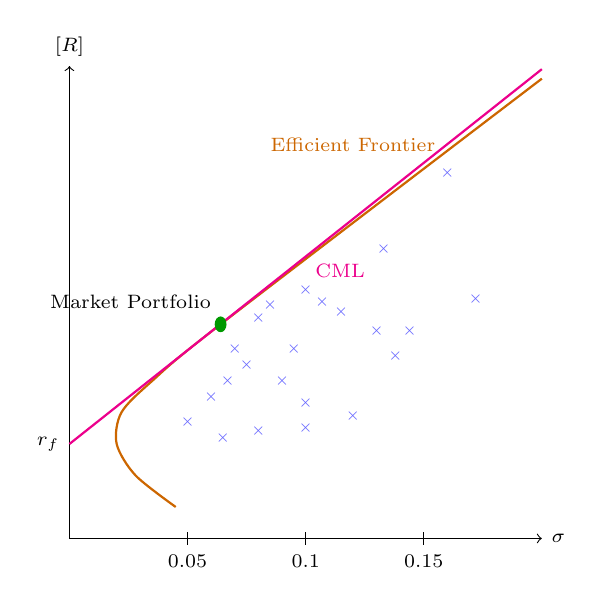
\begin{tikzpicture}[xscale=30, yscale=40]
        \draw[->] (0,0) -- (0.2,0) node[right] {\scriptsize $\sigma$};
        \draw[->] (0,0) -- (0,0.15) node[above] {\scriptsize $\E[R]$};
        \foreach \x in {0.05,0.1,0.15}{\draw (\x,0.002) -- (\x,-0.002) node[below] {\scriptsize \x};}
        \foreach \p in {(0.05,0.037),(0.06,0.045),(0.067,0.05),(0.07,0.06),(0.075,0.055),(0.08,0.07),(0.085,0.074),(0.09,0.05),(0.095,0.06),(0.1,0.079),(0.1,0.043),(0.107,0.075),(0.115,0.072),(0.12,0.039),(0.13,0.066),(0.133,0.092),(0.138,0.058),(0.144,0.066),(0.16,0.116),(0.172,0.076),(0.1,0.035),(0.08,0.034),(0.065,0.032)}
            {\node[blue!60,font=\tiny] at \p {$\times$};}
        \draw[thick,orange!80!black] plot[smooth] coordinates {(0.045,0.01) (0.028,0.02) (0.02,0.03) (0.022,0.04) (0.035,0.05) (0.064,0.068) (0.2,0.146)};
        \draw[thick,magenta] (0,0.03) -- (0.2,0.149);
        \fill[green!60!black] (0.064,0.068) circle (0.0025);
        \node[left,font=\scriptsize] at (0,0.03) {$r_f$};
        \node[above left,font=\scriptsize] at (0.064,0.07) {Market Portfolio};
        \node[font=\scriptsize,orange!80!black] at (0.12,0.125) {Efficient Frontier};
        \node[font=\scriptsize,magenta,right] at (0.1,0.085) {CML};
    \end{tikzpicture}
\end{center}
\begin{itemize}
    \item \rb{Efficient frontier}: the best expected return achievable for each volatility using portfolios of risky assets
    \item \rb{Capital market line (CML)}: the line from $r_f$ tangent to the frontier. The tangent point is the \rb{market portfolio (MP)}
    \item Mixing the MP with lending/borrowing at $r_f$ reaches any point on the CML, which beats the frontier everywhere else
\end{itemize}

\begin{example}[Leveraging Up the CML]
    $r_f = 3\%$, $\E[R_{MP}] = 7\%$, $\sigma_{MP} = 0.06$. Invest \$100 in the
    MP, then borrow another \$50 at $r_f$ and invest it in the MP too.
    \\\db{You hold 1.5$\times$ your wealth in the MP:}
    \[\sigma_p = 1.5\,\sigma_{MP} = 0.09, \qquad \E[R_p] = 1.5(7\% - 3\%) + 3\% = \db{9\%}\]
\end{example}

\heading{Systematic vs.\ Idiosyncratic Risk}
Regress a company's return on the market's:
\[R_{C,t} = \alpha_C + \beta_C' R_{MP,t} + \varepsilon_{C,t}\]
\begin{itemize}
    \item Volatility in $R_{MP,t}$ is \rb{systematic} (``market'') risk
    \item Volatility in $\varepsilon_{C,t}$ is \rb{idiosyncratic} (``firm-specific'') risk
    \item Investors can ``diversify away'' idiosyncratic risk with portfolios, so there is \b{no reward} for bearing it. Investors are only rewarded for market risk, measured by $\beta$
\end{itemize}

\begin{definition}[CAPM]
    The expected return of the $i$-th asset is
    \[\boxed{\E[R_i] = r_f + \beta_i\big(\E[R_{MP}] - r_f\big)}, \qquad
    \beta_i = \frac{\sigma_{i,MP}}{\sigma_{MP}^2} = \frac{\rho_{i,MP}\,\sigma_i}{\sigma_{MP}}\]
    $\E[R_{MP}] - r_f$ is the \rb{market risk premium}. The MP is often
    estimated with a stock index.
\end{definition}

\begin{center}
    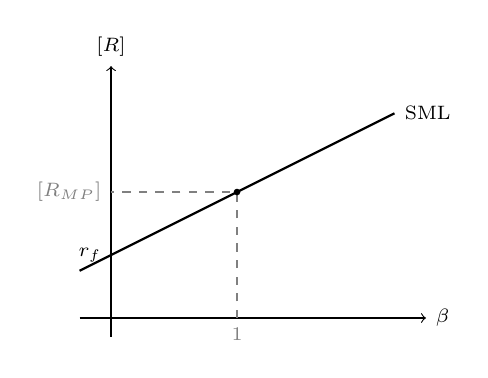
\begin{tikzpicture}[scale=0.8]
        \draw[->] (-0.5,0) -- (5,0) node[right] {\scriptsize $\beta$};
        \draw[->] (0,-0.3) -- (0,4) node[above] {\scriptsize $\E[R]$};
        \draw[thick] (-0.5,0.75) -- (4.5,3.25) node[right] {\scriptsize SML};
        \node[left] at (0,1) {\scriptsize $r_f$};
        \draw[dashed,gray] (2,0) node[below] {\scriptsize 1} -- (2,2) -- (0,2) node[left] {\scriptsize $\E[R_{MP}]$};
        \fill (2,2) circle (1.5pt);
    \end{tikzpicture}
    \\[2pt] \textit{\small Security market line: intercept $r_f$, slope $\E[R_{MP}] - r_f$}
\end{center}

\begin{example}[Estimating Stock Return]
    Market: $r_f = 2\%$, $\E[R_{MP}] = 8\%$, $\sigma_{MP} = 10\%$. Company X:
    correlation to the market $0.6$, volatility $0.15$. Estimate X's
    expected return.
    \[\beta_X = \frac{0.6 \times 0.15}{0.10} = 0.9\]
    \[\E[R_X] = 2\% + 0.9(8\% - 2\%) = \db{7.4\%}\]
    \db{(The handwritten slide used 10\% for the market return, giving 9.2\%. With the stated 8\% it is 7.4\%.)}
\end{example}

\begin{example}[Estimating Future Stock Price]
    A company with $\beta = 0.9$ trades at \$170/share. $r_f = 2\%$, market
    rate $= 7\%$. What is the expected share price in 5 years if it pays no
    dividends?
    \[\E[R_C] = 2\% + 0.9(7\% - 2\%) = 6.5\%\]
    \[P_5 = P_0 e^{\E[R_C]\,t} = 170e^{0.065 \times 5} = \db{\$235}\]
\end{example}

\begin{example}[Reflection: Stock with Dividends]
    A stock trades at \$10 and pays quarterly dividends of \$0.10/share.
    $\E[R_{MP}] = 10\%$, $r_f = 3\%$, $\beta = 1.2$. What is the expected
    price 3 years from now?
    \[\E[R_C] = 3\% + 1.2(10\% - 3\%) = 11.4\%/\text{yr}\]
    \db{Dividends are quarterly, so convert: $(1 + i_q)^4 = 1.114 \Rightarrow i_q = 2.736\%$. Today's price is the PV of 12 dividends plus the price at year 3:}
    \[10 = 0.10(P/A,2.736\%,12) + P_3(P/F,11.4\%,3) \;\Rightarrow\; P_3 = \db{\$12.43}\]
\end{example}

\topic{Arbitrage}

\begin{definition}[Arbitrage]
    \begin{itemize}
        \item \b{In financial markets}: taking advantage of a price difference between two or more markets
        \item \b{Academic use}: an opportunity to achieve a \b{risk-free} gain at a rate \b{greater than the risk-free rate}
        \item \rb{Statistical arbitrage}: a gain at a higher rate than one should get for a given level of risk
    \end{itemize}
    Fundamental to finance theory (and to valuation) is the
    \rb{no-arbitrage assumption}: ``no free lunch''.
\end{definition}

\begin{example}[Corn Arbitrage]
    You can buy a bushel of corn for \$10 today and enter a forward contract
    to deliver it for \$12 one year from now (storage is free). You can also
    borrow at 10\%. What would you do?
    \\\db{Borrow $\$10x$ and buy $x$ bushels today: net cash-flow \$0. In one year, sell the $x$ bushels for $\$12x$ and repay the $\$11x$ loan: a risk-free profit of $\$1x$.}
    \\\db{As $x \to \infty$ the profit is infinite. In reality, demand for corn today pushes the price up until the arbitrage disappears. The no-arbitrage price is}
    \[\frac{\$12}{1.10} = \db{\$10.91}\]
\end{example}

\heading{Futures and Forwards}
\begin{itemize}
    \item Contracts used to \b{hedge} against risks or to \b{speculate}
    \item Examples of \rb{derivative} assets: their value derives from an underlying asset
    \item Both lock in a specific price for a certain asset
\end{itemize}

\begin{definition}[Forward Contract]
    An obligation to buy or sell a certain asset at a specified price (the
    \rb{forward price}) at a specified time (the \rb{maturity} or expiration
    date). Typically not traded on exchanges; both buyer and seller are
    obligated to fulfill their end at maturity.
\end{definition}

\begin{definition}[Futures Contract]
    The same as a forward, except futures are \b{settled daily} (so they can
    be bought or sold at any time) and are traded on a \b{standardized
    exchange}.
\end{definition}

\begin{center}
    \begin{tabular}{ll}
        \toprule
        Futures & Forwards \\
        \midrule
        Settled daily & Settled at maturity \\
        Standardized & Not standardized \\
        Low risk of non-fulfilment (regulated) & Low regulation/oversight on settlement \\
        Traded on public exchanges & Private contract between two parties \\
        \bottomrule
    \end{tabular}
\end{center}
\db{E.g.\ the WTI oil futures curve: the price today for oil delivered in month 1, 2, \dots\ (in March 2020 the curve rose steeply from \$25 to \$45).}

\begin{example}[Interest Rate Forward]
    Given a yield curve $r(t)$, find the forward rate $r_{1,2}$ that one
    could lock in today for borrowing/lending from $t_1$ to $t_2$.
    \\\db{Invest $P_0$ today. Directly to $t_2$: $F_2 = P_0e^{r_{0,2}t_2}$. Or to $t_1$ then roll at the forward rate: $F_2' = P_0e^{r_{0,1}t_1}e^{r_{1,2}(t_2 - t_1)}$. No arbitrage requires $F_2' = F_2$:}
    \[\boxed{r_{1,2} = \frac{r_{0,2}t_2 - r_{0,1}t_1}{t_2 - t_1}}\]
\end{example}

\begin{example}[Foreign Exchange Forward]
    Canadian risk-free rate 3\%, US risk-free rate 2.5\%, current
    FX $= 0.9$ US\$/C\$. What is the fair one-year forward FX rate?
    \\\db{Two risk-free ways to turn C\$1 today into money in one year must agree:}
    \begin{itemize}
        \item \db{Keep it in C\$: $1 \times 1.03 = \text{C}\$1.03$}
        \item \db{Convert to US\$0.90, invest: $0.90 \times 1.025 = \text{US}\$0.9225$}
    \end{itemize}
    \[FX_1 = \frac{\text{US}\$0.9225}{\text{C}\$1.03} = \db{0.896 \text{ US\$/C\$}}\]
\end{example}

\heading{Using Replication to Price an Asset}
Build a portfolio of assets we can already price that has the \b{same
payoff in every state}. By no-arbitrage, the asset's price equals the
portfolio's price.

\begin{example}[Pricing a Project by Replication]
    A project pays \$140 if the market goes up and \$30 if it goes down.
    The risk-free rate is 5\% for the period; the MP is \$100 today and will be
    worth \$120 (up) or \$95 (down). What is a fair price for the project?
    \begin{center}
        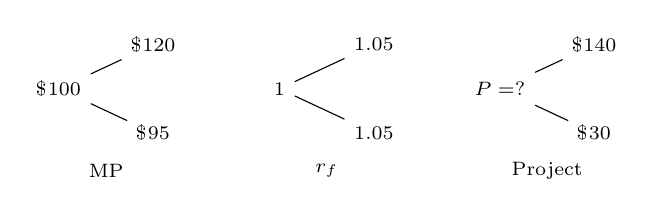
\begin{tikzpicture}[scale=0.8, every node/.style={font=\scriptsize}]
            \node (m) at (0,0) {\$100}; \node (mu) at (1.5,0.7) {\$120}; \node (md) at (1.5,-0.7) {\$95};
            \draw (m) -- (mu); \draw (m) -- (md); \node at (0.75,-1.3) {MP};
            \node (r) at (3.5,0) {1}; \node (ru) at (5,0.7) {1.05}; \node (rd) at (5,-0.7) {1.05};
            \draw (r) -- (ru); \draw (r) -- (rd); \node at (4.25,-1.3) {$r_f$};
            \node (p) at (7,0) {$P = ?$}; \node (pu) at (8.5,0.7) {\$140}; \node (pd) at (8.5,-0.7) {\$30};
            \draw (p) -- (pu); \draw (p) -- (pd); \node at (7.75,-1.3) {Project};
        \end{tikzpicture}
    \end{center}
    \db{Hold $a$ units of the MP and $b$ units of the risk-free asset:}
    \begin{align*}
        \text{Up: } & 120a + 1.05b = 140\\
        \text{Down: } & 95a + 1.05b = 30
    \end{align*}
    \db{$\Rightarrow a = 4.4$, $b = -369.52$ (borrow).}
    \[P = 100(4.4) - 1(369.52) = \db{\$70.48}\]
    \db{Note that we did \dbb{not} use the probabilities!}
\end{example}

\begin{example}[Expected Returns and the Project's Beta]
    Same setup; the probability the market goes up is 60\%.
    \[\E[R_{MP}] = \frac{120(0.6) + 95(0.4)}{100} - 1 = 10\%\]
    \[\E[R_{proj}] = \frac{140(0.6) + 30(0.4)}{70.48} - 1 = 36.2\%\]
    \db{Back out the project's beta from CAPM:}
    \[36.2\% = 5\% + \beta_{proj}(10\% - 5\%) \;\Rightarrow\; \beta_{proj} = \db{6.24}\]
    \db{The project swings far more than the market, so it is heavily ``leveraged'' market risk.}
\end{example}

\begin{example}[Payoffs Independent of the Market]
    \begin{enumerate}[label = \alph*)]
        \item What if the project paid \$140 regardless of what the market did?
        \\\db{It is risk-free: $P = 140/1.05 = \$133$.}
        \item What if the payoff had a 50\% chance of being \$150 and 50\% of being \$130 (independent of the market)?
        \\\db{$\E[\text{payoff}] = 0.5(150) + 0.5(130) = \$140$. The risk is purely idiosyncratic (diversifiable), so it carries no premium: $P = 140/1.05 = \$133$.}
    \end{enumerate}
\end{example}

\begin{example}[Systematic and Idiosyncratic Risk]
    A wealthy (risk-neutral) investor can invest in a product development
    project. There is a 60\% chance the technology works very well
    (independent of the market). Payoffs:
    \begin{center}
    \begin{tabular}{lcc}
        \toprule
        & Tech works (60\%) & Doesn't (40\%) \\
        \midrule
        Market up & \$80k & \$50k \\
        Market down & \$55k & \$20k \\
        \bottomrule
    \end{tabular}
    \end{center}
    The MP is \$45 today, worth \$60 (up) or \$40 (down); $r_f = 5\%$. An
    initial R\&D investment of \$20k is required. What is the maximum price
    for the project?
    \\\db{The technology risk is idiosyncratic, so replace it by its expectation in each market state:}
    \[\E[P_u] = 0.6(80k) + 0.4(50k) = 68k, \qquad \E[P_d] = 0.6(55k) + 0.4(20k) = 41k\]
    \db{Replicate the market risk:}
    \begin{align*}
        60a + 1.05b &= 68k\\
        40a + 1.05b &= 41k
    \end{align*}
    \db{$\Rightarrow a = 1.35k$, $b = -12.38k$.}
    \[P_0 = 1.35k(45) - 12.38k = \$48.37k\]
    \db{Since \$20k of R\&D is also needed, buy the project for \dbb{\$28.37k or less}.}
\end{example}

\begin{example}[Bond: Accounting for Default]
    A company issues a 5-year bond (face \$100) with a 5\% annual coupon.
    The \b{risk-neutral probability} of default in any given year is 5\%,
    and on default only half of the principal (\$50) is paid out. The
    risk-free rate is 3\%.
    \begin{enumerate}[label = \alph*)]
        \item What is the probability of default over the 5 years?
        \\\db{$1 - 0.95^5 = 22.6\%$}
        \item What should the price of the bond be?
        \\\db{Work backwards through the tree. Each year the bond either survives (95\%, pays the coupon plus the value going forward) or defaults (5\%, pays \$50). Discount each step at $r_f$ since these are risk-neutral probabilities:}
        \begin{align*}
            P_{up}^{(4)} &= 5 + \frac{0.95(105) + 0.05(50)}{1.03} = 104.27\\
            P_{up}^{(3)} &= 5 + \frac{0.95(104.27) + 0.05(50)}{1.03} = 103.60\\
            P_{up}^{(2)} &= 5 + \frac{0.95(103.60) + 0.05(50)}{1.03} = 102.98\\
            P_{up}^{(1)} &= 5 + \frac{0.95(102.98) + 0.05(50)}{1.03} = 102.41\\
            P_0 &= \frac{0.95(102.41) + 0.05(50)}{1.03} = \db{\$96.88}
        \end{align*}
        \item What is the yield?
        \[96.88 = 5(P/A,y,5) + 100(P/F,y,5) \;\Rightarrow\; y = \db{5.735\%}\]
        \db{The yield is above the 3\% risk-free rate (and the 5\% coupon) to compensate for default risk.}
    \end{enumerate}
\end{example}

\heading{Summary}
\begin{enumerate}
    \item Risk is the uncertainty in a future payoff; investors demand a higher expected return for bearing it
    \item Only \b{systematic} (market) risk is rewarded. CAPM: $\E[R_i] = r_f + \beta_i(\E[R_{MP}] - r_f)$
    \item \b{No arbitrage}: two ways to get the same payoff must cost the same. This prices forwards (corn, interest rates, FX)
    \item \b{Replication}: match an asset's payoffs with the MP and the risk-free asset; the price does not need the real-world probabilities
\end{enumerate}
